% !Mode:: "TeX:UTF-8"
\documentclass[12pt,a4paper]{article}

%%%%%%%%------------------------------------------------------------------------
%%%% 日常所用宏包

%% 控制页边距
% 如果是beamer文档类, 则不用geometry
\makeatletter
\@ifclassloaded{beamer}{}{\usepackage[top=2.5cm, bottom=2.5cm, left=2.5cm, right=2.5cm]{geometry}}
\makeatother

%% 控制项目列表
\usepackage{enumerate}

%% 多栏显示
\usepackage{multicol}

%% 算法环境
\usepackage{algorithm}  
\usepackage{algorithmic} 
\usepackage{float} 

%% 网址引用
\usepackage{url}

%% 控制矩阵行距
\renewcommand\arraystretch{1.4}

%% hyperref宏包,生成可定位点击的超链接,并且会生成pdf书签
\makeatletter
\@ifclassloaded{beamer}{
\usepackage{hyperref}
\usepackage{ragged2e} % 对齐
}{
\usepackage[%
    pdfstartview=FitH,%
    CJKbookmarks=true,%
    bookmarks=true,%
    bookmarksnumbered=true,%
    bookmarksopen=true,%
    colorlinks=true,%
    citecolor=blue,%
    linkcolor=blue,%
    anchorcolor=green,%
    urlcolor=blue%
]{hyperref}
}
\makeatother



\makeatletter % 如果是 beamer 不需要下面两个包
\@ifclassloaded{beamer}{
\mode<presentation>
{
} 
}{
%% 控制标题
\usepackage{titlesec}
%% 控制目录
\usepackage{titletoc}
}
\makeatother

%% 控制表格样式
\usepackage{booktabs}

%% 控制字体大小
\usepackage{type1cm}

%% 首行缩进,用\noindent取消某段缩进
\usepackage{indentfirst}

%% 支持彩色文本、底色、文本框等
\usepackage{color,xcolor}

%% AMS LaTeX宏包: http://zzg34b.w3.c361.com/package/maths.htm#amssymb
\usepackage{amsmath,amssymb}
%% 多个图形并排
\usepackage{subfig}
%%%% 基本插图方法
%% 图形宏包
\usepackage{graphicx}
\newcommand{\red}[1]{\textcolor{red}{#1}}
\newcommand{\blue}[1]{\structure{#1}}
\newcommand{\brown}[1]{\textcolor{brown}{#1}}
\newcommand{\green}[1]{\textcolor{green}{#1}}


%%%% 基本插图方法结束

%%%% pgf/tikz绘图宏包设置
\usepackage{pgf,tikz}
\usetikzlibrary{shapes,automata,snakes,backgrounds,arrows}
\usetikzlibrary{mindmap}
%% 可以直接在latex文档中使用graphviz/dot语言,
%% 也可以用dot2tex工具将dot文件转换成tex文件再include进来
%% \usepackage[shell,pgf,outputdir={docgraphs/}]{dot2texi}
%%%% pgf/tikz设置结束


\makeatletter % 如果是 beamer 不需要下面两个包
\@ifclassloaded{beamer}{

}{
%%%% fancyhdr设置页眉页脚
%% 页眉页脚宏包
\usepackage{fancyhdr}
%% 页眉页脚风格
\pagestyle{plain}
}

%% 有时会出现\headheight too small的warning
\setlength{\headheight}{15pt}

%% 清空当前页眉页脚的默认设置
%\fancyhf{}
%%%% fancyhdr设置结束


\makeatletter % 对 beamer 要重新设置
\@ifclassloaded{beamer}{

}{
%%%% 设置listings宏包用来粘贴源代码
%% 方便粘贴源代码,部分代码高亮功能
\usepackage{listings}

%% 设置listings宏包的一些全局样式
%% 参考http://hi.baidu.com/shawpinlee/blog/item/9ec431cbae28e41cbe09e6e4.html
\lstset{
showstringspaces=false,              %% 设定是否显示代码之间的空格符号
numbers=left,                        %% 在左边显示行号
numberstyle=\tiny,                   %% 设定行号字体的大小
basicstyle=\footnotesize,                    %% 设定字体大小\tiny, \small, \Large等等
keywordstyle=\color{blue!70}, commentstyle=\color{red!50!green!50!blue!50},
                                     %% 关键字高亮
frame=shadowbox,                     %% 给代码加框
rulesepcolor=\color{red!20!green!20!blue!20},
escapechar=`,                        %% 中文逃逸字符,用于中英混排
xleftmargin=2em,xrightmargin=2em, aboveskip=1em,
breaklines,                          %% 这条命令可以让LaTeX自动将长的代码行换行排版
extendedchars=false                  %% 这一条命令可以解决代码跨页时,章节标题,页眉等汉字不显示的问题
}}
\makeatother
%%%% listings宏包设置结束


%%%% 附录设置
\makeatletter % 对 beamer 要重新设置
\@ifclassloaded{beamer}{

}{
\usepackage[title,titletoc,header]{appendix}
}
\makeatother
%%%% 附录设置结束


%%%% 日常宏包设置结束
%%%%%%%%------------------------------------------------------------------------


%%%%%%%%------------------------------------------------------------------------
%%%% 英文字体设置结束
%% 这里可以加入自己的英文字体设置
%%%%%%%%------------------------------------------------------------------------

%%%%%%%%------------------------------------------------------------------------
%%%% 设置常用字体字号,与MS Word相对应

%% 一号, 1.4倍行距
\newcommand{\yihao}{\fontsize{26pt}{36pt}\selectfont}
%% 二号, 1.25倍行距
\newcommand{\erhao}{\fontsize{22pt}{28pt}\selectfont}
%% 小二, 单倍行距
\newcommand{\xiaoer}{\fontsize{18pt}{18pt}\selectfont}
%% 三号, 1.5倍行距
\newcommand{\sanhao}{\fontsize{16pt}{24pt}\selectfont}
%% 小三, 1.5倍行距
\newcommand{\xiaosan}{\fontsize{15pt}{22pt}\selectfont}
%% 四号, 1.5倍行距
\newcommand{\sihao}{\fontsize{14pt}{21pt}\selectfont}
%% 半四, 1.5倍行距
\newcommand{\bansi}{\fontsize{13pt}{19.5pt}\selectfont}
%% 小四, 1.5倍行距
\newcommand{\xiaosi}{\fontsize{12pt}{18pt}\selectfont}
%% 大五, 单倍行距
\newcommand{\dawu}{\fontsize{11pt}{11pt}\selectfont}
%% 五号, 单倍行距
\newcommand{\wuhao}{\fontsize{10.5pt}{10.5pt}\selectfont}
%%%%%%%%------------------------------------------------------------------------


%% 设定段间距
\setlength{\parskip}{0.5\baselineskip}

%% 设定行距
\linespread{1}


%% 设定正文字体大小
% \renewcommand{\normalsize}{\sihao}

%制作水印
\RequirePackage{draftcopy}
\draftcopyName{XTUMESH}{100}
\draftcopySetGrey{0.90}
\draftcopyPageTransform{40 rotate}
\draftcopyPageX{350}
\draftcopyPageY{80}

%%%% 个性设置结束
%%%%%%%%------------------------------------------------------------------------


%%%%%%%%------------------------------------------------------------------------
%%%% bibtex设置

%% 设定参考文献显示风格
% 下面是几种常见的样式
% * plain: 按字母的顺序排列,比较次序为作者、年度和标题
% * unsrt: 样式同plain,只是按照引用的先后排序
% * alpha: 用作者名首字母+年份后两位作标号,以字母顺序排序
% * abbrv: 类似plain,将月份全拼改为缩写,更显紧凑
% * apalike: 美国心理学学会期刊样式, 引用样式 [Tailper and Zang, 2006]

\makeatletter
\@ifclassloaded{beamer}{
\bibliographystyle{apalike}
}{
\bibliographystyle{unsrt}
}
\makeatother


%%%% bibtex设置结束
%%%%%%%%------------------------------------------------------------------------

%%%%%%%%------------------------------------------------------------------------
%%%% xeCJK相关宏包

\usepackage{xltxtra,fontspec,xunicode}
\usepackage[slantfont, boldfont]{xeCJK} 

%% 针对中文进行断行
\XeTeXlinebreaklocale "zh"             

%% 给予TeX断行一定自由度
\XeTeXlinebreakskip = 0pt plus 1pt minus 0.1pt

%%%% xeCJK设置结束                                       
%%%%%%%%------------------------------------------------------------------------

%%%%%%%%------------------------------------------------------------------------
%%%% xeCJK字体设置

%% 设置中文标点样式,支持quanjiao、banjiao、kaiming等多种方式
\punctstyle{kaiming}                                        
                                                     
%% 设置缺省中文字体
\setCJKmainfont[BoldFont={Adobe Heiti Std}, ItalicFont={Adobe Kaiti Std}]{Adobe Song Std}   
%% 设置中文无衬线字体
\setCJKsansfont[BoldFont={Adobe Heiti Std}]{Adobe Kaiti Std}  
%% 设置等宽字体
\setCJKmonofont{Adobe Heiti Std}                            

%% 英文衬线字体
\setmainfont{DejaVu Serif}                                  
%% 英文等宽字体
\setmonofont{DejaVu Sans Mono}                              
%% 英文无衬线字体
\setsansfont{DejaVu Sans}                                   

%% 定义新字体
\setCJKfamilyfont{song}{Adobe Song Std}                     
\setCJKfamilyfont{kai}{Adobe Kaiti Std}
\setCJKfamilyfont{hei}{Adobe Heiti Std}
\setCJKfamilyfont{fangsong}{Adobe Fangsong Std}
\setCJKfamilyfont{lisu}{LiSu}
\setCJKfamilyfont{youyuan}{YouYuan}

%% 自定义宋体
\newcommand{\song}{\CJKfamily{song}}                       
%% 自定义楷体
\newcommand{\kai}{\CJKfamily{kai}}                         
%% 自定义黑体
\newcommand{\hei}{\CJKfamily{hei}}                         
%% 自定义仿宋体
\newcommand{\fangsong}{\CJKfamily{fangsong}}               
%% 自定义隶书
\newcommand{\lisu}{\CJKfamily{lisu}}                       
%% 自定义幼圆
\newcommand{\youyuan}{\CJKfamily{youyuan}}                 

%%%% xeCJK字体设置结束
%%%%%%%%------------------------------------------------------------------------

%%%%%%%%------------------------------------------------------------------------
%%%% 一些关于中文文档的重定义
\newcommand{\chntoday}{\number\year\,年\,\number\month\,月\,\number\day\,日}
%% 数学公式定理的重定义

%% 中文破折号,据说来自清华模板
\newcommand{\pozhehao}{\kern0.3ex\rule[0.8ex]{2em}{0.1ex}\kern0.3ex}

\newtheorem{example}{例}                                   
\newtheorem{theorem}{定理}[section]                         
\newtheorem{definition}{定义}
\newtheorem{axiom}{公理}
\newtheorem{property}{性质}
\newtheorem{proposition}{命题}
\newtheorem{lemma}{引理}
\newtheorem{corollary}{推论}
\newtheorem{remark}{注解}
\newtheorem{condition}{条件}
\newtheorem{conclusion}{结论}
\newtheorem{assumption}{假设}

\makeatletter %
\@ifclassloaded{beamer}{

}{
%% 章节等名称重定义
\renewcommand{\contentsname}{目录}     
\renewcommand{\indexname}{索引}
\renewcommand{\listfigurename}{插图目录}
\renewcommand{\listtablename}{表格目录}
\renewcommand{\appendixname}{附录}
\renewcommand{\appendixpagename}{附录}
\renewcommand{\appendixtocname}{附录}
%% 设置chapter、section与subsection的格式
\titleformat{\chapter}{\centering\huge}{第\thechapter{}章}{1em}{\textbf}
\titleformat{\section}{\centering\sihao}{\thesection}{1em}{\textbf}
\titleformat{\subsection}{\xiaosi}{\thesubsection}{1em}{\textbf}
\titleformat{\subsubsection}{\xiaosi}{\thesubsubsection}{1em}{\textbf}

\@ifclassloaded{book}{

}{
\renewcommand{\abstractname}{摘要}
}
}
\makeatother

\renewcommand{\figurename}{图}
\renewcommand{\tablename}{表}

\makeatletter
\@ifclassloaded{book}{
\renewcommand{\bibname}{参考文献}
}{
\renewcommand{\refname}{参考文献} 
}
\makeatother

\floatname{algorithm}{算法}
\renewcommand{\algorithmicrequire}{\textbf{输入:}}
\renewcommand{\algorithmicensure}{\textbf{输出:}}

%%%% 中文重定义结束
%%%%%%%%------------------------------------------------------------------------


\title{重心坐标与基函数}
\author{}
\date{\chntoday}

\begin{document}
\maketitle

\section{重心坐标}
重心坐标是构造基函数的基础,所以首先引入重心坐标。知道一个点的重心坐标后,就可以知道它在单元中的位置。

数学中,重心坐标是由单纯形(如三角形或四面体等)顶点定义的坐标,不局限于具体的坐标系。单纯形中的点由单纯形各顶点线性表出,组合系数便是重心坐标。下面定义重心坐标。

令 $P$ 是一个 $n$ 维空间中的单纯形,其顶点记为 $\lbrace X_i=(x_{i,0},x_{i,1},\cdots ,x_{i,n-1})\rbrace_{i=0,\cdots,n}$,~$n\ge 1$,且满足右手法则(平面上满足逆时针顺序)。对任意的 $X=(x_0 ,x_1,\cdots ,x_{n-1})^T\in P$,定义函数 $\lambda _i(X):P\longrightarrow R,~i=0,\cdots,n$.若
$$
X=\sum_{i=0}^n \lambda _i(X)X_i,~\sum_{i=0}^n\lambda _i(X)\equiv 1.
$$
则称 $\lambda _i(X)$ 为齐次坐标,$\lambda _0(x),\lambda _1(x),\cdots,\lambda _n(x)$ 中只有 $n$ 个自由量。此外,若 $\lambda _i(X)\ge 0,~i=0,\cdots,n$,则称 $\lambda _i(X)$ 为重心坐标。显然可以将上式看作一个以 $\lambda _i(X)$ 为未知量,$X$ 和 $X_i$ 为已知量的非齐次线性方程组,那么,
$$\begin{bmatrix}
x_{0,0} & x_{1,0} & \cdots & x_{n,0}\\
x_{0,1} & x_{1,1} & \cdots & x_{n,1}\\
\vdots & \ddots & \vdots \\
x_{0,n-1} & x_{1,n-1} & \cdots & x_{n,n-1}\\
1 & 1 & \cdots & 1\\
\end{bmatrix}
\begin{bmatrix}
\lambda _0 \\
\lambda _1 \\
\vdots \\
\lambda _{n-1} \\
\lambda _n \\
\end{bmatrix}=
\begin{bmatrix}
x _0 \\
x _1 \\
\vdots \\
x _{n-1} \\
1 \\
\end{bmatrix}$$

从而重心坐标是上述方程组的非负解,由系数矩阵 
$\begin{bmatrix}
x_{0,0} & x_{1,0} & \cdots & x_{n,0}\\
x_{0,1} & x_{1,1} & \cdots & x_{n,1}\\
\vdots & \ddots & \vdots \\
x_{0,n-1} & x_{1,n-1} & \cdots & x_{n,n-1}\\
1 & 1 & \cdots & 1\\
\end{bmatrix}$ 的非奇异可知,$\lambda _0,\lambda _1,\cdots ,\lambda _n$ 存在唯一。

一维的区间$[x_0,x_1]$

$$
\begin{cases}
\lambda _0(x)x_0+\lambda _1(x)x_1=x,\\
\lambda _0(x)+\lambda _1(x)=1.
\end{cases}
$$
即
$$
\begin{bmatrix}
x_0 & x_1 \\
1 & 1 \\
\end{bmatrix}
\begin{bmatrix}
\lambda _0(x)\\
\lambda _1(x)\\
\end{bmatrix}=\begin{bmatrix}
x\\
1\\
\end{bmatrix}.
$$
由 $\begin{bmatrix}
x_0 & x_1 \\
1 & 1 \\
\end{bmatrix}$ 的非奇异可知,$\lambda _0(x)$,$\lambda _1(x)$ 存在唯一。

重心坐标的几何意义:

\begin{figure}[H]
\centering

\includegraphics[scale=0.7]{./figures/1.png}
\caption{}
\end{figure}

任取$P$属于该区间,则

$$\lambda _0 =\frac{PX_1}{X_0 X_1},\quad \lambda _1 =\frac{X_0 P}{X_0 X_1}.$$

二维的三角形
$$
\begin{cases}
\lambda _0(X)x_0+\lambda _1(X)x_1+\lambda _2(X)x_2=x,\\
\lambda _0(X)y_0+\lambda _1(X)y_1+\lambda _2(X)y_2=y,\\
\lambda _0(X)+\lambda _1(X)+\lambda _2(X)=1.
\end{cases}
$$
即
$$
\begin{bmatrix}
x_0 & x_1 & x_2\\
y_0 & y_1 & y_2\\
1 & 1 & 1\\
\end{bmatrix}
\begin{bmatrix}
\lambda _0(X)\\
\lambda _1(X)\\
\lambda _2(X)\\
\end{bmatrix}=\begin{bmatrix}
x\\
y\\
1\\
\end{bmatrix}.
$$
由 $\begin{bmatrix}
x_0 & x_1 & x_2\\
y_0 & y_1 & y_2\\
1 & 1 & 1\\
\end{bmatrix}$ 的非奇异可知,$\lambda _0(X)$,$\lambda _1(X)$,$\lambda _2(X)$ 存在唯一。

重心坐标的几何意义:

\begin{figure}[H]
\centering
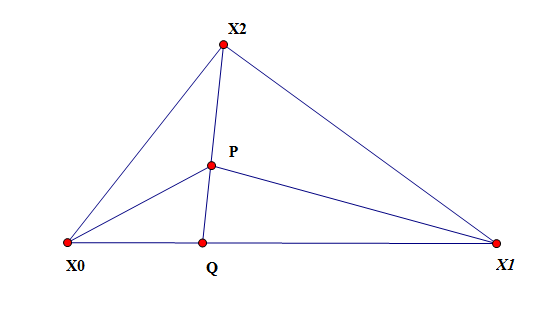
\includegraphics[scale=0.7]{./figures/2.png}
\caption{}
\end{figure}

任取 $P\in \triangle_{X_0 X_1 X_2}$,延长 $X_2 P$ 使之与 $X_0 X_1$ 相交于点 $Q$,则
$$
\lambda _2=\frac {PQ}{X_2 Q}=\frac{S_{\triangle PX_0 X_1}}{S_{\triangle X_0 X_1 X_2}}.
$$

重心坐标表示 $P$ 在三角形单元内的位置,三角形单元所在的系统平移或者旋转都不会对重心坐标的值产生影响。

三维的四面体
$$
\begin{cases}
\lambda _0(X)x_0+\lambda _1(X)x_1+\lambda _2(X)x_2+\lambda _3(X)x_3=x,\\
\lambda _0(X)y_0+\lambda _1(X)y_1+\lambda _2(X)y_2+\lambda _3(X)y_3=y,\\
\lambda _0(X)z_0+\lambda _1(X)z_1+\lambda _2(X)z_2+\lambda _3(X)z_3=z,\\
\lambda _0(X)+\lambda _1(X)+\lambda _2(X)+\lambda _3(X)=1.
\end{cases}
$$
即
$$
\begin{bmatrix}
x_0 & x_1 & x_2 & x_3\\
y_0 & y_1 & y_2 & y_3\\
z_0 & z_1 & z_2 & z_3\\
1 & 1 & 1 &1\\
\end{bmatrix}
\begin{bmatrix}
\lambda _0(X)\\
\lambda _1(X)\\
\lambda _2(X)\\
\lambda _3(X)\\
\end{bmatrix}=\begin{bmatrix}
x\\
y\\
z\\
1\\
\end{bmatrix}.
$$
由 $\begin{bmatrix}
x_0 & x_1 & x_2 & x_3\\
y_0 & y_1 & y_2 & y_3\\
z_0 & z_1 & z_2 & z_3\\
1 & 1 & 1 &1\\
\end{bmatrix}$ 的非奇异可知,$\lambda _0(X)$,$\lambda _1(X)$,$\lambda _2(X)$,$\lambda _3(X)$ 存在唯一。

重心坐标的几何意义:
\begin{figure}[H]
\centering
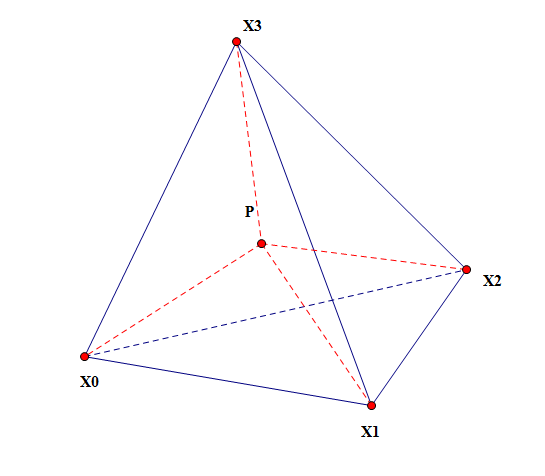
\includegraphics[scale=0.7]{./figures/8.png}
\caption{}
\end{figure}

任取 $P$属于四面体$X_0 X_1 X_2 X_3$,连接 $X_0 ,X_1 ,X_2 ,X_3$,则
$$
\lambda _0=\frac {dist(P,X_0 X_1 X_2)}{dist(X_3,X_0 X_1 X_2)}=\frac{V_{P X_0 X_1 X_2}}{V_{X_0 X_1 X_2 X_3}}.
$$

\section{Silvester插值多项式}
这里我们先介绍Silvester插值多项式,再通过Silvester插值多项式构造基函数,Silvester插值多项式定义为
$$
R_i (p,\lambda)=\begin{cases}
\frac{1}{i!}\prod_{k=0}^{i-1} (p\lambda-k),~& 1\leqslant i\leqslant p\\
1,& i=0\\
\end{cases}
$$
可知这是关于 $\lambda$ 的 $i$ 次多项式,其中 $\lambda$ 为 $[0,1]$ 中的插值节点,$p$ 表示区间 $[0,1]$ 的等分数,当 $\lambda=0,1/p,2/p,\cdots ,(i-1)/p$ 时 $\frac{1}{i!}\prod_{k=0}^{i-1} (p\lambda-k) =0$,当 $\lambda=i/p$ 时 $\frac{1}{i!}\prod_{k=0}^{i-1} (p\lambda-k) =1.$

利用Silvester插值多项式就可以构造出高次的有限元单元的基函数。增加有限元单元的基函数的次数可以提高精度,但不是次数越高越好,因为如果次数过高,计算的误差积累反而会使精度下降。

\section{单纯形上的基函数}
区间 $[x_0,x_1]$ 上 $p$ 次拉格朗日基函数的构造

首先构造一维区间 $[x_0,x_1]$ 上的重心坐标,
$$
\begin{cases}
\lambda _0(x)x_0+\lambda _1(x)x_1=x,\\
\lambda _0(x)+\lambda _1(x)=1.
\end{cases}
$$
则,
$$
\begin{bmatrix}
x_0 & x_1\\
1 & 1\\
\end{bmatrix}
\begin{bmatrix}
\lambda _0(x)\\
\lambda _1(x)\\
\end{bmatrix}=\begin{bmatrix}
x\\
1\\
\end{bmatrix},
$$
因此,
$$
\lambda _0(x)=\frac{\begin{vmatrix}
x & x_1 \\
1 & 1 \\
\end{vmatrix}}{\begin{vmatrix}
x_0 & x_1 \\
1 & 1 \\
\end{vmatrix}}=\frac{x-x_1}{x_0-x_1}=\frac{x_1-x}{x_1-x_0},
\quad\lambda _1(x)=\frac{\begin{vmatrix}
x_0 & x \\
1 & 1
\end{vmatrix}}{\begin{vmatrix}
x_0 & x_1 \\
1 & 1
\end{vmatrix}}=\frac{x_0-x}{x_0-x_1}=\frac{x-x_0}{x_1-x_0}.
$$
$\forall ~x\in [x_0,x_1]$,则 $\lambda _0(x)\ge 0$,~$\lambda _1(x)\ge 0$.并且
$$
\begin{cases}
\lambda _0 (x_0)=1,\quad\lambda _0 (x_1)=0,\\
\lambda _1 (x_0)=0,\quad\lambda _1 (x_1)=1.\\
\end{cases}
$$
易知, $\lambda_0, \lambda_1$ 都是关于 $x$ 的线性函数(这里指一次函数)。

也可以通过下面的方式计算重心坐标。

设 $\lambda_0 (x)=ax+b$,则
$$
\begin{cases}
\lambda _0 (x_0)=ax_0+b=1,\\
\lambda _0 (x_1)=ax_1+b=0.\\
\end{cases}
$$
从而可以求出 $a$,$b$,进而求出 $\lambda _0$.同理可得 $\lambda _1$.

重心坐标关于 $x$ 的导数为:
$$
\frac{\mathrm d \lambda_0}{\mathrm dx} = -\frac{1}{x_1 - x_0},\quad 
\frac{\mathrm d \lambda_1}{\mathrm dx} = \frac{1}{x_1 - x_0}.
$$
区间 $[x_0, x_1]$ 上的 $p\geq 1$ 次基函数共有 
$n_{dof} = p+1$ 个,其 $p$ 次插值基函数的计算公式如下:
$$
\phi_{m,n}= \frac{1}{m!}\prod_{l_0 = 0}^{m - 1}(p\lambda_0 -l_0)\frac{1}{n!}\prod_{l_1 = 0}^{n - 1}(p\lambda_1 -l_1)
$$
即
$$
\phi_{m,n}= R_m (p,\lambda_0)R_n (p,\lambda_1).
$$

其中 $m\geq 0$, $n\geq 0$, 且 $m+n=p$,即 $\phi_{m,n}$ 是一个 $p$ 次多项式。

由 $\lambda_0=\frac{x_1 - x}{x_1 - x_0}=\frac{l_0}{p}$ 得到
$$
x=x_1-\frac{l_0}{p} (x_1 - x_0)=(1-\frac{l_0}{p})x_1 + \frac{l_0}{p} x_0,\quad l_0=0,1,\cdots ,(m-1).
$$
因为 $(1-\frac{l_0}{p}) + \frac{l_0}{p} =1$,故 $x\in [x_0,x_1].$

由 $\lambda_1=\frac{x - x_0}{x_1 - x_0}=\frac{l_1}{p}$ 得到
$$
x=x_0+\frac{l_1}{p} (x_1 - x_0)=\frac{l_1}{p} x_1 + (1-\frac{l_1}{p})x_0,\quad l_1=0,1,\cdots ,(n-1).
$$
因为 $(1-\frac{l_1}{p}) + \frac{l_1}{p} =1$,故 $x\in [x_0,x_1].$

因此 $p$ 次插值基函数过节点 $x_1,\frac{(p-1)x_1 + x_0}{p},\frac{(p-2)x_1 + 2x_0}{p},\frac{(p-3)x_1 + 3x_0}{p},\cdots,x_0$,即把区间均匀等分,步长为 $\frac{(x_1-x_0)}{p}$.

要在区间上构造一个 $p$ 次基函数,需要确定 $p+1$ 个系数,即需要 $p+1$ 个节点,从而需要把区间$p$等分。

这个 $p$ 次插值基函数实际上就是这种形式的
$$
l_k(x)=\frac{(x-x_0)\cdots(x-x_{k-1})(x-x_{k+1})\cdots(x - x_p)}{(x_k-x_0)\cdots(x_k-x_{k-1})(x_k-x_{k+1})\cdots(x_k-x_p)}
$$
拉格朗日插值基函数的特殊化形式。

$p$ 次基函数的面向数组的计算

构造向量:
$$
P = ( \frac{1}{0!},  \frac{1}{1!}, \frac{1}{2!}, \cdots, \frac{1}{p!})
$$

构造矩阵:
$$
A :=                                                                            
\begin{pmatrix}  
1  &  1  \\
p\lambda_0 & p\lambda_1\\                                             
p\lambda_0 - 1 & p\lambda_1 - 1\\   
\vdots & \vdots \\                                                     
p\lambda_0 - (p - 1) & \lambda_1 - (p - 1)
\end{pmatrix}                                                                   
$$ 
对 $A$ 的每一列做累乘运算,并左乘由 $P$ 形成的对角矩阵,得矩阵:

$$
B = \mathrm{diag}(P)
\begin{pmatrix}
1 & 1\\
p\lambda_0 & p\lambda_1\\
\prod_{l=0}^{1}(p\lambda_0 - l) & \prod_{l=0}^{1}(p\lambda_1 - l)\\
\vdots & \vdots \\
\prod_{l=0}^{p-1}(p\lambda_0 - l) & \prod_{l=0}^{p-1}(p\lambda_1 - l) 
\end{pmatrix}
$$

易知,只需从 $B$ 的每一列中各选择一项相乘(要求二项次数之和为 $p$),即可得到相应的基函数,其中取法共有 

$$
n_{dof} = {p+1}
$$

构造指标矩阵:

$$
I = \begin{pmatrix}
p  & 0 \\ p-1 & 1 \\ \vdots & \vdots \\ 0 & p 
\end{pmatrix}
$$
由$I$可知一共有$\begin{matrix} p+1 \\ \overbrace{ 1+1+\cdots+1 }
\end{matrix}$种选择。

\section{三角形单元}
下面考虑二维三角形单元的重心坐标。

给定三角形单元 $\tau$, 其三个顶点 $X_0 :=(x_0,y_0)$, $X_1 :=(x_1,y_1)$ 和 $X_2 :=(x_2,y_2)$ 逆时针排列,且不在同一条直线上,那么向量 $\overrightarrow{X_0 X_1}$ 和 $\overrightarrow{X_0 X_2}$ 是线性无关的。这等价于矩阵

$$
A = 
\begin{pmatrix}
x_0 & x_1 & x_2 \\
y_0 & y_1 & y_2 \\
1   & 1   & 1 
\end{pmatrix}
$$

非奇异。
又 $|A|\ne 0$,故任给一点 $X:=(x,y)\in\tau$,下面的线性方程组

$$
A 
\begin{pmatrix}
\lambda_0 \\
\lambda_1\\
\lambda_2  
\end{pmatrix}
=\begin{pmatrix}
x \\
y\\
1  
\end{pmatrix}
$$

有唯一的一组解 $\lambda_0,\lambda_1,\lambda_2$. 
因此对任意二维点 $X\in\tau$, 有
$$
\begin{cases}
\lambda _0 x_0+\lambda _1 x_1+\lambda _2 x_2=x,\\
\lambda _0 y_0+\lambda _1 y_1+\lambda _2 y_2=y,\\
\lambda _0+ \lambda _1 +\lambda _2 =1.
\end{cases}
$$
故$\lambda _0 (x_0,y_0)+\lambda _1 (x_1,y_1)+\lambda _2 (x_2,y_2)=(x,y)$,
从而
$$
X=\lambda_0(X) X_0 + \lambda_1(X)X_1 + \lambda_2(X)X_2 
\text{ 且 } \lambda_0(X) + \lambda_1(X) + \lambda_2(X) = 1. 
$$

$\lambda_0,\lambda_1,\lambda_2$ 称为点 $X$ 关于点 $X_0,X_1$ 和$X_2$ 的重心坐标。

易知, $\lambda_0, \lambda_1, \lambda_2$ 都是关于 $X$ 的线性函数,且有

\begin{eqnarray*}
\lambda_0(X_0) = 1,\quad & \lambda_0(X_1) = 0,\quad& \lambda_0(X_2) = 0\\
\lambda_1(X_0) = 0,\quad & \lambda_1(X_1) = 1,\quad& \lambda_1(X_2) = 0\\
\lambda_2(X_0) = 0,\quad & \lambda_2(X_1) = 0,\quad & \lambda_2(X_2) = 1\\
\end{eqnarray*}

\begin{figure}[H]
\centering
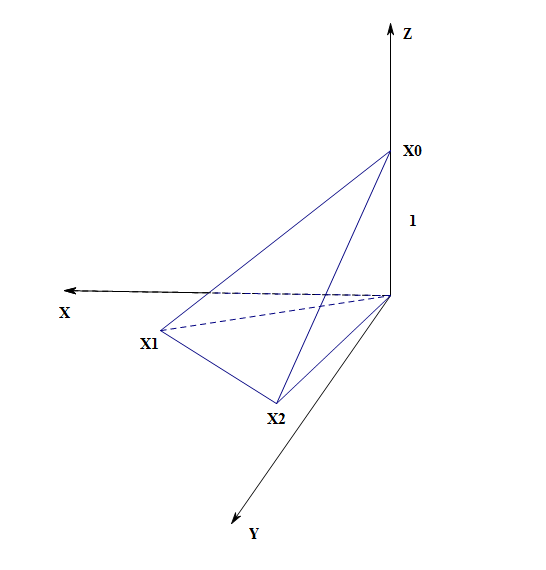
\includegraphics[scale=0.7]{./figures/3.png}
\caption{}
\end{figure}

也可以通过下面的方式计算重心坐标。

设 $\lambda_0 (x,y)=ax+by+c$,则
$$
\begin{cases}
\lambda _0 (x_0,y_0)=ax_0+by_0+c=1,\\
\lambda _0 (x_1,y_1)=ax_1+by_1+c=0,\\
\lambda _0 (x_2,y_2)=ax_2+by_2+c=0.\\
\end{cases}
$$
从而可以求出 $a$,$b$,$c$,进而求出 $\lambda _0$.同理可得 $\lambda _1$,$\lambda _2$.

为了考虑变化率的大小和方向,引入梯度。梯度的大小是变化率最大的值,梯度的方向是变化率最大的方向。

$\lambda_0, \lambda_1, \lambda_2$ 关于 $X$ 的梯度分别为:

$$
\begin{aligned}
\nabla\lambda_0 = \frac{1}{2|\tau|}(X_2 - X_1)W\\
\nabla\lambda_1 = \frac{1}{2|\tau|}(X_0 - X_2)W\\
\nabla\lambda_2 = \frac{1}{2|\tau|}(X_1 - X_0)W\\
\end{aligned}
$$

其中 

$$
W = \begin{pmatrix}
0 & 1\\ -1 & 0 
\end{pmatrix}
$$
三角形单元上的 $p$ 次基函数公式

给定三角形单元上的一个重心坐标 $(\lambda_0, \lambda_1, \lambda_2)$, 所有 $p\geq 1$ 次基函数的计算公式如下:
$$
\phi_{m,n,k} =\frac{1}{m!}\prod_{l_0 = 0}^{m - 1}(p\lambda_0 - l_0)\frac{1}{n!}\prod_{l_1 = 0}^{n - 1}(p\lambda_1 - l_1)\frac{1}{k!}\prod_{l_2 = 0}^{k - 1}(p\lambda_2 - l_2).
$$

即
$$
\phi_{m,n,k} =R_m (p,\lambda_0)R_n (p,\lambda_1)R_k (p,\lambda_2).
$$
其中 $ m\geq 0$, $n\geq 0$, $ k \geq 0$, 且 $m+n+k=p$.

三角形单元上的 $p$ 次基函数面向矩阵计算

构造向量:
$$
P = ( \frac{1}{0!},  \frac{1}{1!}, \frac{1}{2!}, \cdots, \frac{1}{p!})
$$

构造矩阵:
$$
A :=                                                                            
\begin{pmatrix}  
1  &  1  & 1 \\
p\lambda_0 & p\lambda_1 & p\lambda_2\\                                             
p\lambda_0 - 1 & p\lambda_1 - 1 & p\lambda_2 - 1\\   
\vdots & \vdots & \vdots \\                                                     
p\lambda_0 - (p - 1) & p\lambda_1 - (p - 1) & p\lambda_2 - (p - 1)
\end{pmatrix}                                                                   
$$ 
对 $A$ 的每一列做累乘运算,并左乘由 $P$ 形成的对角矩阵,得矩阵:

$$
B = \mathrm{diag}(P)
\begin{pmatrix}
1 & 1 & 1 \\
p\lambda_0 & p\lambda_1 & p\lambda_2\\
\prod_{l=0}^{1}(p\lambda_0 - l) & \prod_{l=0}^{1}(p\lambda_1 - l)
& \prod_{l=0}^{1}(p\lambda_2 - l) \\
\vdots & \vdots & \vdots \\
\prod_{l=0}^{p-1}(p\lambda_0 - l) & \prod_{l=0}^{p-1}(p\lambda_1 - l)
& \prod_{l=0}^{p-1}(p\lambda_2 - l) 
\end{pmatrix}
$$
易知,只需从 $B$ 的每一列中各选择一项相乘(要求三项次数之和为 $p$),即可得到相应的基函数,其中取法共有 
$$
n_{dof} = \frac{(p+1)(p+2)}{2}
$$
即需要构造 $n_{dof}\times 3$ 的指标矩阵 $I$, 

$$
I = \begin{pmatrix}
p & 0 & 0 \\
p-1 & 1 & 0 \\
p-1 & 0 & 1 \\
p-2 & 2 & 0 \\
p-2 & 1 & 1 \\
p-2 & 0 & 2 \\
\vdots & \vdots & \vdots \\
0   & p & 0 \\
0   & p-1 & 1\\
\vdots & \vdots & \vdots \\
0   & 0  & p
\end{pmatrix}
$$
由 $I$ 可知一共有 $1+2+3+\cdots+(p+1)=\frac{(p+1)(p+2)}{2}$ 种选择。

这里我们将三角形单元的边分成 $2$ 等分,再平行各边连线,得到下图
\begin{figure}[H]
\centering
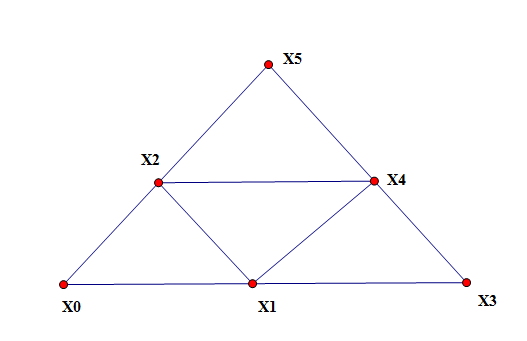
\includegraphics[scale=0.7]{./figures/9.png}
\caption{}
\end{figure}
一个节点对应一个基函数,上图中一共有 $6$ 个节点,因此一共有 $6$ 个基函数,由上面的 $p$ 次基函数计算公式得到三角形单元上的全部 $2$ 次基函数集合$\lbrace \frac{1}{2!}2\lambda_0 (2\lambda_0 -1),\frac{1}{2!}2\lambda_1 (2\lambda_1 -1),\frac{1}{2!}2\lambda_2 (2\lambda_2 -1),(2\lambda_0)(2\lambda_1),(2\lambda_0)(2\lambda_2),(2\lambda_1)(2\lambda_2)\rbrace $.

我们首先看 $X_0$ 对应的基函数 $M$,$M(X_0)=1$,其它点$M$ 等于 $0$.线段 $X_3 X_5$ 对应的是函数 $\lambda _0=0$,$X_1 X_2$ 对应的是函数 $\lambda _0=\frac{1}{2}$,因此$\lambda_0 (X_3), \lambda_0 (X_4), \lambda_0 (X_5)=0$,$\lambda_0 (X_1), \lambda_0 (X_2)=\frac{1}{2}$.因此$M=\frac{1}{2!}2\lambda_0 (2\lambda_0 -1)$.

$X_0 X_5$ 对应的是函数 $\lambda _1=0$,$X_1 X_4$ 对应的是函数 $\lambda _1=\frac{1}{2}$,因此$\lambda_1 (X_0), \lambda_1 (X_2), \lambda_1 (X_5)=0$,$\lambda_1 (X_1), \lambda_1 (X_4)=\frac{1}{2}$.

$X_0 X_3$ 对应的是函数 $\lambda _2=0$,$X_2 X_4$ 对应的是函数 $\lambda _2=\frac{1}{2}$,因此$\lambda_2 (X_0), \lambda_2 (X_1), \lambda_2 (X_3)=0$,$\lambda_2 (X_2), \lambda_2 (X_4)=\frac{1}{2}$.

综上,$X_1$ 对应的基函数是 $(2\lambda_0)(2\lambda_1)$,$X_2$ 对应的基函数是 $(2\lambda_0)(2\lambda_2)$,$X_3$ 对应的基函数是 $\frac{1}{2!}2\lambda_1 (2\lambda_1 -1)$,$X_4$ 对应的基函数是 $(2\lambda_1)(2\lambda_2)$,$X_5$ 对应的基函数是 $\frac{1}{2!}2\lambda_2 (2\lambda_2 -1)$.

要在二维三角形单元中确定以 $p$ 次基函数,需要确定 $\frac{(p+1)(p+2)}{2}$ 个系数,即需要 $\frac{(p+1)(p+2)}{2}$ 个节点,这里我们将三角形单元的边分成 $p$ 等分,再平行各边连线,以 $p=3$ 为例,如下图
\begin{figure}[H]
\centering
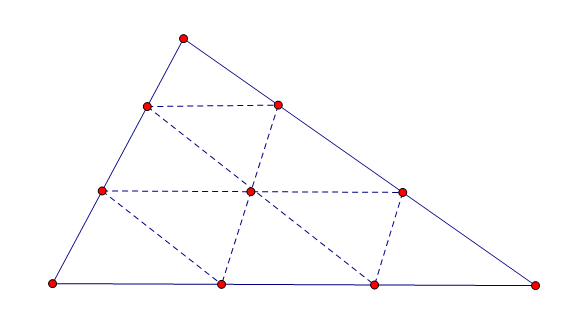
\includegraphics[scale=0.7]{./figures/4.png}
\caption{}
\end{figure}



\section{四面体单元}
给定四面体单元 $\tau$, 其三个顶点 $X_0 :=(x_0, y_0,z_0)$, $X_1 :=(x_1,y_1,z_1)$, $X_2 :=(x_2,y_2,z_2)$ 和 $X_3 :=(x_3, y_3, z_3)$ 排列满足右手法则, 体积不为零. 这等价于矩阵

$$
A = 
\begin{pmatrix}
x_0 & x_1 & x_2 & x_3\\
y_0 & y_1 & y_2 & y_3\\
z_0 & x_1 & x_2 & x_3\\
1   & 1   & 1 & 1
\end{pmatrix}
$$

非奇异. 

任给一点 $X=(x,y)\in\tau$, 求解下面的线性方程组

$$
A 
\begin{pmatrix}
\lambda_0 \\
\lambda_1\\
\lambda_2 \\
\lambda_3
\end{pmatrix}
=\begin{pmatrix}
x \\
y\\
z \\
1  
\end{pmatrix}
$$

可得唯一的一组解$\lambda_0,\lambda_1,\lambda_2, \lambda_3$. 

因此对任意三维点 $X\in\tau$, 有

$$
X=\lambda_0(X)X_0 + \lambda_1(X)X_1 + \lambda_2(X)X_2 + \lambda_3(X)X_3 
\text{ 且 } \lambda_0(X) + \lambda_1(X) + \lambda_2(X) + \lambda_3(X) = 1. 
$$

$\lambda_0,\lambda_1,\lambda_2, \lambda_3$ 称为点 $X$ 关于点 $X_0$, $X_1$, $X_2$, $X_3$ 的重心坐标。
易知, $\lambda_0, \lambda_1, \lambda_2, \lambda_3$ 都是关于 $X$ 的线性函数,并且

$$
\lambda_0(X_0) = 1,\quad \lambda_0(X_1) = 0,\quad \lambda_0(X_2) = 0,\quad \lambda_0(X_3) = 0
$$
$$\lambda_1(X_0) = 0,\quad \lambda_1(X_1) = 1,\quad \lambda_1(X_2) = 0,\quad \lambda_0(X_3) = 0
$$
$$
\lambda_2(X_0) = 0,\quad \lambda_2(X_1) = 0,\quad \lambda_2(X_2) = 1,\quad \lambda_0(X_3) = 0
$$
$$
\lambda_3(X_0) = 0,\quad \lambda_3(X_1) = 0,\quad \lambda_3(X_2) = 0,\quad \lambda_0(X_3) = 1
$$

也可以通过下面的方式计算重心坐标。

设 $\lambda_0 (x,y,z)=ax+by+cz+d$,则
$$
\begin{cases}
\lambda _0 (x_0,y_0,z_0)=ax_0+by_0+cz_0+d=1,\\
\lambda _0 (x_1,y_1,z_1)=ax_1+by_1+cz_1+d=0,\\
\lambda _0 (x_2,y_2,z_2)=ax_2+by_2+cz_2+d=0,\\
\lambda _0 (x_3,y_3,z_3)=ax_3+by_3+cz_3+d=0.\\
\end{cases}
$$
从而可以求出 $a$,$b$,$c$,$d$,进而求出 $\lambda _0$.同理可得 $\lambda _1$,$\lambda _2$,$\lambda _3$.

三维情形的基函数表示如下:
$$
\phi_{m,n,k,v} = \frac{1}{m!}\prod_{l_0 = 0}^{m - 1}
(p\lambda_0 -l_0)\frac{1}{n!}\prod_{l_1 = 0}^{n-1}(p\lambda_1 -
l_1)\frac{1}{k!}\prod_{l_2=0}^{k-1}(p\lambda_2 -l_2)\frac{1}{v!}\prod_{l_3=0}^{v-1}(p\lambda_3 - l_3).
$$
即
$$
\phi_{m,n,k,v} =R_m (p,\lambda_0)R_n (p,\lambda_1)R_k (p,\lambda_2)R_v (p,\lambda_3)
$$



其中 $ m\geq 0$, $n\geq 0$, $ k \geq 0$, $v\geq 0$,  且 $m+n+k+v=p$.

构造向量:
$$
P = ( \frac{1}{0!},  \frac{1}{1!}, \frac{1}{2!}, \cdots, \frac{1}{p!})
$$

构造矩阵:
$$
A :=                                                                            
\begin{pmatrix}  
1  &  1  & 1 & 1\\
p\lambda_0 & p\lambda_1 & p\lambda_2 & p\lambda_3\\                                             
p\lambda_0 - 1 & p\lambda_1 - 1 & p\lambda_2 - 1 & p\lambda_3 - 1\\   
\vdots & \vdots & \vdots & \vdots \\                                                     
p\lambda_0 - (p - 1) & p\lambda_1 - (p - 1) & p\lambda_2 - (p - 1) & p\lambda_3 - (p - 1)
\end{pmatrix}                                                                   
$$ 

对 $A$ 的每一列做累乘运算,并左乘由 $P$ 形成的对角矩阵,得矩阵:

$$
B = \mathrm{diag}(P)
\begin{pmatrix}
1 & 1 & 1 & 1\\
p\lambda_0 & p\lambda_1 & p\lambda_2 & p\lambda_3\\
\prod_{l=0}^{1}(p\lambda_0 - l) & \prod_{l=0}^{1}(p\lambda_1 - l)
& \prod_{l=0}^{1}(p\lambda_2 - l) & \prod_{l=0}^{1}(p\lambda_3 - l) \\
\vdots & \vdots & \vdots & \vdots \\
\prod_{l=0}^{p-1}(p\lambda_0 -l) & \prod_{l=0}^{p-1}(p\lambda_1 - l)
& \prod_{l=0}^{p-1}(p\lambda_2 - l) & \prod_{l=0}^{p-1}(p\lambda_3 - l) 
\end{pmatrix}
$$
易知,只需从 $B$ 的每一列中各选择一项相乘(要求四项次数之和为 $p$),即可得到相应的基函数,其中取法共有 

$$
n_{dof} = \frac{(p+1)(p+2)(p+3)}{6}
$$
即需要构造 $n_{dof}\times 3$ 的指标矩阵 $I$, 

$$
I = \begin{pmatrix}
p & 0 & 0 & 0\\
p-1 & 1 & 0 & 0\\
p-1 & 0 & 1 & 0\\
p-1 & 0 & 0 & 1\\
p-2 & 2 & 0 & 0\\
p-2 & 1 & 1 & 0\\
p-2 & 1 & 0 & 1\\
p-2 & 0 & 2 & 0 \\
p-2 & 0 & 1 & 1 \\
p-2 & 0 & 0 & 2\\
\vdots & \vdots & \vdots & \vdots \\
0   & p & 0 & 0 \\
0   & p-1 & 1 & 0\\
\vdots & \vdots & \vdots & \vdots \\
0   & 0  & 0 & p 
\end{pmatrix}
$$
由 $I$ 可知一共有 $1+3+6+10+15+21+28+\cdots+(p+1)=\frac{(p+1)(p+2)(p+3)}{6}$ 种选择。

要在三维四面体单元中确定以 $p$ 次基函数,需要确定 $\frac{(p+1)(p+2)(p+3)}{6}$ 个系数,即需要 $\frac{(p+1)(p+2)(p+3)}{6}$ 个节点。

\section{四边形单元}
给定一个四边形单元 $\tau := (X_0, X_1, X_2, X_3)$, 可以建立它与参考单元之间的映射关系

$$
A :=
\begin{pmatrix}
1 - \xi \\
\xi
\end{pmatrix}
\begin{pmatrix}
1 - \eta & \eta
\end{pmatrix}
= 
\begin{pmatrix}
(1-\xi)(1-\eta) & (1-\xi)\eta\\
\xi(1-\eta) & \xi\eta
\end{pmatrix}
$$

$$
X(\xi, \eta) =
\begin{pmatrix}
(1-\xi)(1-\eta) & (1-\xi)\eta & \xi(1-\eta) & 
\xi\eta
\end{pmatrix}
\begin{pmatrix}
x_0 \\ x_1 \\ x_2 \\ x_3
\end{pmatrix}=
A\begin{pmatrix}
x_0 \\ x_1 \\ x_2 \\ x_3
\end{pmatrix}
$$

$$
\begin{pmatrix}
\frac{\mathrm d x}{\mathrm d \xi} & \frac{\mathrm d x}{\mathrm d\eta}\\
\frac{\mathrm d y}{\mathrm d \xi} & \frac{\mathrm d y}{\mathrm d\eta}
\end{pmatrix}
=
\begin{pmatrix}
(\eta - 1)x_0 -\eta x_1 + (1 - \eta) x_2 + \eta x_3 & (\xi - 1)x_0 + (1 - \xi) x_1  - \xi x_2 + \xi x_3\\
(\eta - 1)y_0 -\eta y_1 + (1 - \eta) y_2 + \eta y_3 & (\xi - 1)y_0 + (1 - \xi) y_1  - \xi y_2 + \xi y_3
\end{pmatrix}
$$

$$
\begin{pmatrix}
\frac{\mathrm d x}{\mathrm d \xi} & \frac{\mathrm d x}{\mathrm d\eta}\\
\frac{\mathrm d y}{\mathrm d \xi} & \frac{\mathrm d y}{\mathrm d\eta}
\end{pmatrix}
=
\begin{pmatrix}
x_2 - x_0 & x_1 - x_0\\
y_2 - y_0 & y_1 - y_0
\end{pmatrix}
+
\begin{pmatrix}
x_0 - x_1 - x_2 + x_3\\
y_0 - y_1 - y_2 + y_3
\end{pmatrix}
\begin{pmatrix}
\eta & \xi
\end{pmatrix}
$$

记 $\lambda_0 = 1-x$, $\lambda_1 = x$, 利用上面的方法可以构造 $[0, 1]$ 区间上的一元 $p$ 次基函数

\begin{figure}[H]
\centering
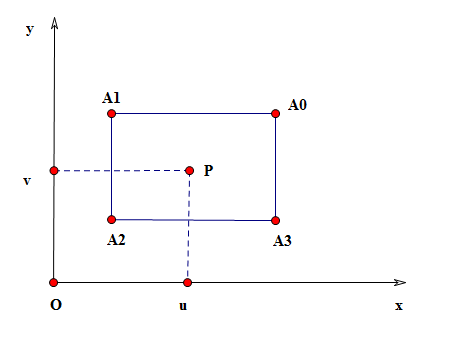
\includegraphics[scale=0.7]{./figures/5.png}
\caption{}
\end{figure}


$$
\Phi(x) = (\phi_0(x), \phi_1(x), \cdots, \phi_{p}(x))
$$

节点 $X_0$ 对应的基函数为 $\phi_0(x)$,节点 $X_1$ 对应的基函数为 $\phi_1(x)$,$\cdots$,节点 $X_p$ 对应的基函数为 $\phi_p(x)$.

可以通过 $\Phi(\xi) \times \Phi(\eta)$ 构造 $[0, 1] \times [0, 1]$ 中的 $2p$ 次基函数。

\begin{figure}[H]
\centering

\includegraphics[scale=0.7]{./figures/6.png}
\caption{}
\end{figure}


参考单元上的双 $p$ 次元基函数为 

$$
\Phi^T(\xi)\Phi(\eta) =
\begin{pmatrix}
\phi_0(\xi)\phi_0(\eta) & \phi_0(\xi)\phi_1(\eta) & \cdots & \phi_0(\xi)\phi_p(\eta)\\
\phi_1(\xi)\phi_0(\eta) & \phi_1(\xi)\phi_1(\eta) & \cdots & \phi_1(\xi)\phi_p(\eta)\\
\vdots & \vdots & \ddots & \vdots \\
\phi_p(\xi)\phi_0(\eta) & \phi_p(\xi)\phi_1(\eta) & \cdots & \phi_p(\xi)\phi_p(\eta)
\end{pmatrix}
$$

梯度的计算公式为

$$
\left(\frac{\mathrm d \Phi^T(\xi)}{\mathrm d \xi}\Phi(\eta), \Phi^T(\xi)\frac{\mathrm d \Phi^T(\eta)}{\mathrm d\eta}\right)
$$

\section{六面体单元}
给定一个六面体单元 $\tau := (x_0, x_1, x_2, x_3, x_4, x_5, x_6, x_7)$, 建立它与参考单元的映射关系。


记 $\lambda_0 = 1-x$, $\lambda_1 = x$, 利用上面的方法可以构造 $[0, 1]$ 区间上的一元 $p$ 次基函数
$$
\Phi(x) = (\phi_0(x), \phi_1(x), \cdots, \phi_{p}(x))
$$
可以通过 $\Phi(\xi) \times \Phi(\eta)\times \Phi(\varepsilon)$ 构造 $[0, 1] \times [0, 1] \times [0, 1]$ 中的 $3p$ 次基函数。

\begin{figure}[H]
\centering
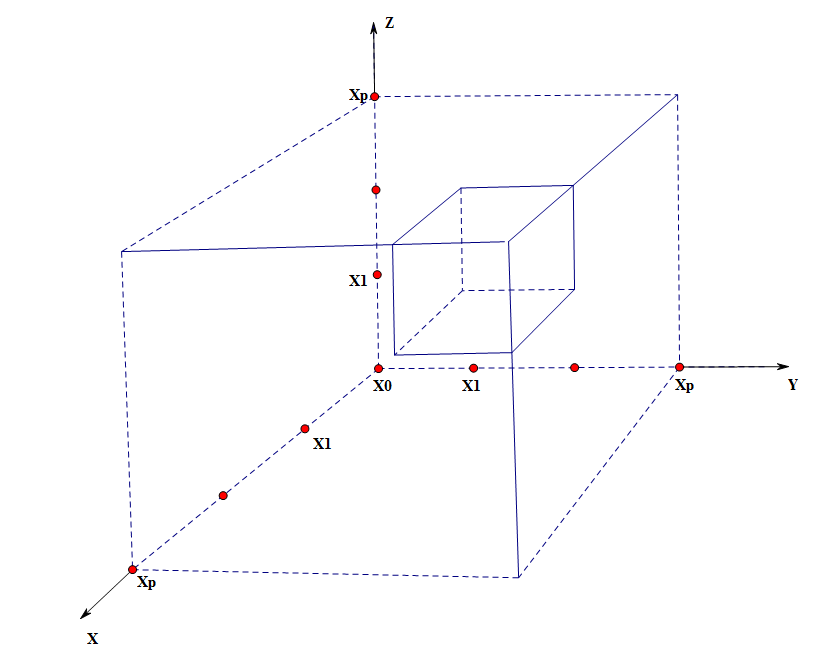
\includegraphics[scale=0.7]{./figures/10.png}
\caption{}
\end{figure}

点 $(X_i ,X_j ,X_k)$ 对应的基函数为 $\phi_i\phi_j\phi_k$.

\section{矢量有限元法}
早起有限元方法,用插值节点数值而获得的节点基函数来表示矢量电场或磁场,可能会有伪解出现,因此产生了矢量有限元法。
这是一种基于单元棱边的有限元法,又称为棱边元法,使用矢量基函数,将自由度赋予棱边而不是单元节点。有限元法可分为节点元法和棱边元法,前面讲的基函数的构造属于节点元法的基函数构造,下面我们讲棱边元法的矢量基函数的构造。
棱边元的有限元法将未知函数定义在棱边上,也就是取场矢量沿棱边的切向分量与棱边长度的乘积作为未知函数,这样能够保证共用一条棱边的相邻单元的切向向量相等。

在构造高阶矢量元的基函数之前,先定义内移Silvester插值多项式
$$
\hat{R}_i (p,L)=R_{i-1}(p,L-1/p)=\begin{cases}
\frac{1}{(i-1)!}\prod_{k=0}^{i-1} (pL-k), & 2 \leqslant i \leqslant p\\
1, & i=1
\end{cases}
$$
由定义可以看出,$i$ 阶内移Silvester插值多项式 $\hat{R}_i (p,L)$ 就是插值点内移的 $i-1$ 阶Silvester插值多项式。

有了Silvester插值多项式和内移Silvester插值多项式,便可以构造高阶矢量元。

对于三角形单元而言,其 $p$ 阶矢量基函数为
$$
N^1_{ijk}=C^1_{ijk}R_i (p+2,L_1)\hat{R}_j (p+2,L_2)\hat{R}_k (p+2,L_3)N_1,i=0,1,\cdots,p;~j,k=1,2,\cdots,p+1
$$
$$
N^2_{ijk}=C^2_{ijk}\hat{R}_i (p+2,L_1)R_j (p+2,L_2)\hat{R}_k (p+2,L_3)N_2,j=0,1,\cdots,p;~i,k=1,2,\cdots,p+1
$$
$$
N^3_{ijk}=C^3_{ijk}\hat{R}_i (p+2,L_1)\hat{R}_j (p+2,L_2)R_k (p+2,L_3)N_3,k=0,1,\cdots,p;~i,j=1,2,\cdots,p+1
$$
这里 $i+j+k=p+2$,$N_1,N_2,N_3$ 是下列没有归一的边缘元基函数
$$
N_1=L_2 \nabla L_3-L_3\nabla L_2
$$
$$
N_2=L_3 \nabla L_1-L_1\nabla L_3
$$
$$
N_1=L_1 \nabla L_2-L_2\nabla L_1
$$
$C^1_{ijk},C^2_{ijk},C^3_{ijk}$ 是归一化系数,以保证基函数 $N^1_{ijk},N^2_{ijk},N^3_{ijk}$ 在插值点处沿 $l_{\beta}$ 方向的切线分量值为 $1$.
$$
C^1_{ijk}=\frac{p+2}{p+2-i}l^{ijk}_1
$$
$$
C^2_{ijk}=\frac{p+2}{p+2-j}l^{ijk}_2
$$
$$
C^3_{ijk}=\frac{p+2}{p+2-k}l^{ijk}_3
$$
$l^{ijk}_{\beta}$ 是 $l_{\beta}=|l_{\beta}|$ 在插值点 $(\frac{i}{p+2},\frac{j}{p+2},\frac{k}{p+2})$ 的取值,$\beta=1,2,3$.



对于四面体单元而言,其 $p$ 阶矢量基函数为
$$
N^1_{ijkl}=C^1_{ijkl}\hat{R}_i (p+2,L_1)\hat{R}_j (p+2,L_2){R}_k (p+2,L_3){R}_l (p+2,L_4)N_1,i,j=1,2,\cdots,p+1;~k,l=0,1,\cdots,p
$$
其中
$$
N_1=L_2 \nabla L_3-L_3 \nabla L_2
$$
$$
C^1_{ijkl}=\frac{p+2}{p+2-i-j}l^(ijkl)_1
$$
这里 $l^(ijkl)_1$ 为 $l_1=|l_1|$ 在插值点 $(\frac{i}{p+2},\frac{j}{p+2},\frac{k}{p+2},\frac{l}{p+2})$ 的值,其他的 $N^{\beta}_{ijkl}$,$\beta =2,3,\cdots,6$ 可以类似得出。




























%\cite{tam19912d}
%\bibliography{../ref}
\end{document}
